\providecommand{\main}{../../../..}
\documentclass[\main/dresen_thesis.tex]{subfiles}

\begin{document}
  \label{sec:monolayers:nanoparticle:edx}

  \begin{table}[ht]
    \centering
    \caption{\label{tab:monolayers:nanoparticles:edx}Ratio of cobalt and iron in the nanoparticles as determined by EDX. Additionally the formula unit that deduce for the acetylacetonate particles from assuming total occupation of the inverse spinell (\ch{Co_x Fe_{3-x} O4}) and from the assumption of only \ch{Fe^{3+}} in the lattice (\ch{Co_x Fe_y O4}) are given. For Ol-CoFe-C the ratio is used to approximate the composition of the w\"ustite phase.}
    \begin{tabular}{ l | r | r | r }
      \textbf{EDX}                & \textbf{Ol-CoFe-C} & \textbf{Ac-CoFe-C} & \textbf{Ac-CoFe-C-2}\\
      \hline
      \rule{0pt}{2ex} $N_{\ch{Fe}} / N_{\ch{Co}}$ & 2.49(27)                   & 3.35(10)                    & 2.67(6)\\
      \hline
      \hline
      \rule{0pt}{2ex}  \ch{Co_x Fe_{3-x} O4}      &                            & \ch{Co_{0.69} Fe_{2.31} O4} & \ch{Co_{0.82} Fe_{2.18} O4}\\
      \rule{0pt}{2ex}  \ch{Co_x Fe_y O4}          &                            & \ch{Co_{0.66} Fe_{2.22} O4} & \ch{Co_{0.80} Fe_{2.13} O4}\\
      \rule{0pt}{2ex}  \ch{Fe_x Co_{1-x} O}       & \ch{Fe_{0.71} Co_{0.29} O} &                             &\\
      \hline
    \end{tabular}
  \end{table}

  The evaluation of the spectra obtained by EDX on large agglomerations of the nanoparticle batches yields the relative compositon in iron and cobalt for the nanoparticle batches as tabulated in \reftab{tab:monolayers:nanoparticles:edx}.
  Ol-CoFe-C has a composition ratio $2.49(27)$, for a feed ratio of $2$.
  Ac-CoFe-C shows a ratio of iron to cobalt of $3.35(10)$, whereas Ac-Co-Fe-C-2 is given by $2.67(6)$.
  This can be compared to the feed ratio of $1.54$ used in Ac-CoFe-C and $1.74$ in Ac-CoFe-C-2.
  This is in contrast to the linear dependence of feed ratio and resulting composition ratio that is observed in literature \cite{Sathya_2016_Cofeo}.

  To explain this discrepancy, the differently chosen heating rates in both synthesis need to be considered.
  The reactants in the acetylacetonates synthesis decompose not exactly equally as can be seen by a thermogravimetric-analysis performed on the chemicals as shown in \reffig{fig:monolayers:nanoparticle:edx:TGARefluxAcAc}.
  The iron acetylacetonate decomposes faster in comparison and therefore, when given more time by a slow heating as was the case in the synthesis of Ac-CoFe-C ($5 \unit{K \, min^{-1}}$) in comparison to Ac-CoFe-C-2  ($15 \unit{K \, min^{-1}}$), the ratio of iron to cobalt monomers is in favor of iron at the growth stage.
  \begin{figure}[tb]
    \centering
    % 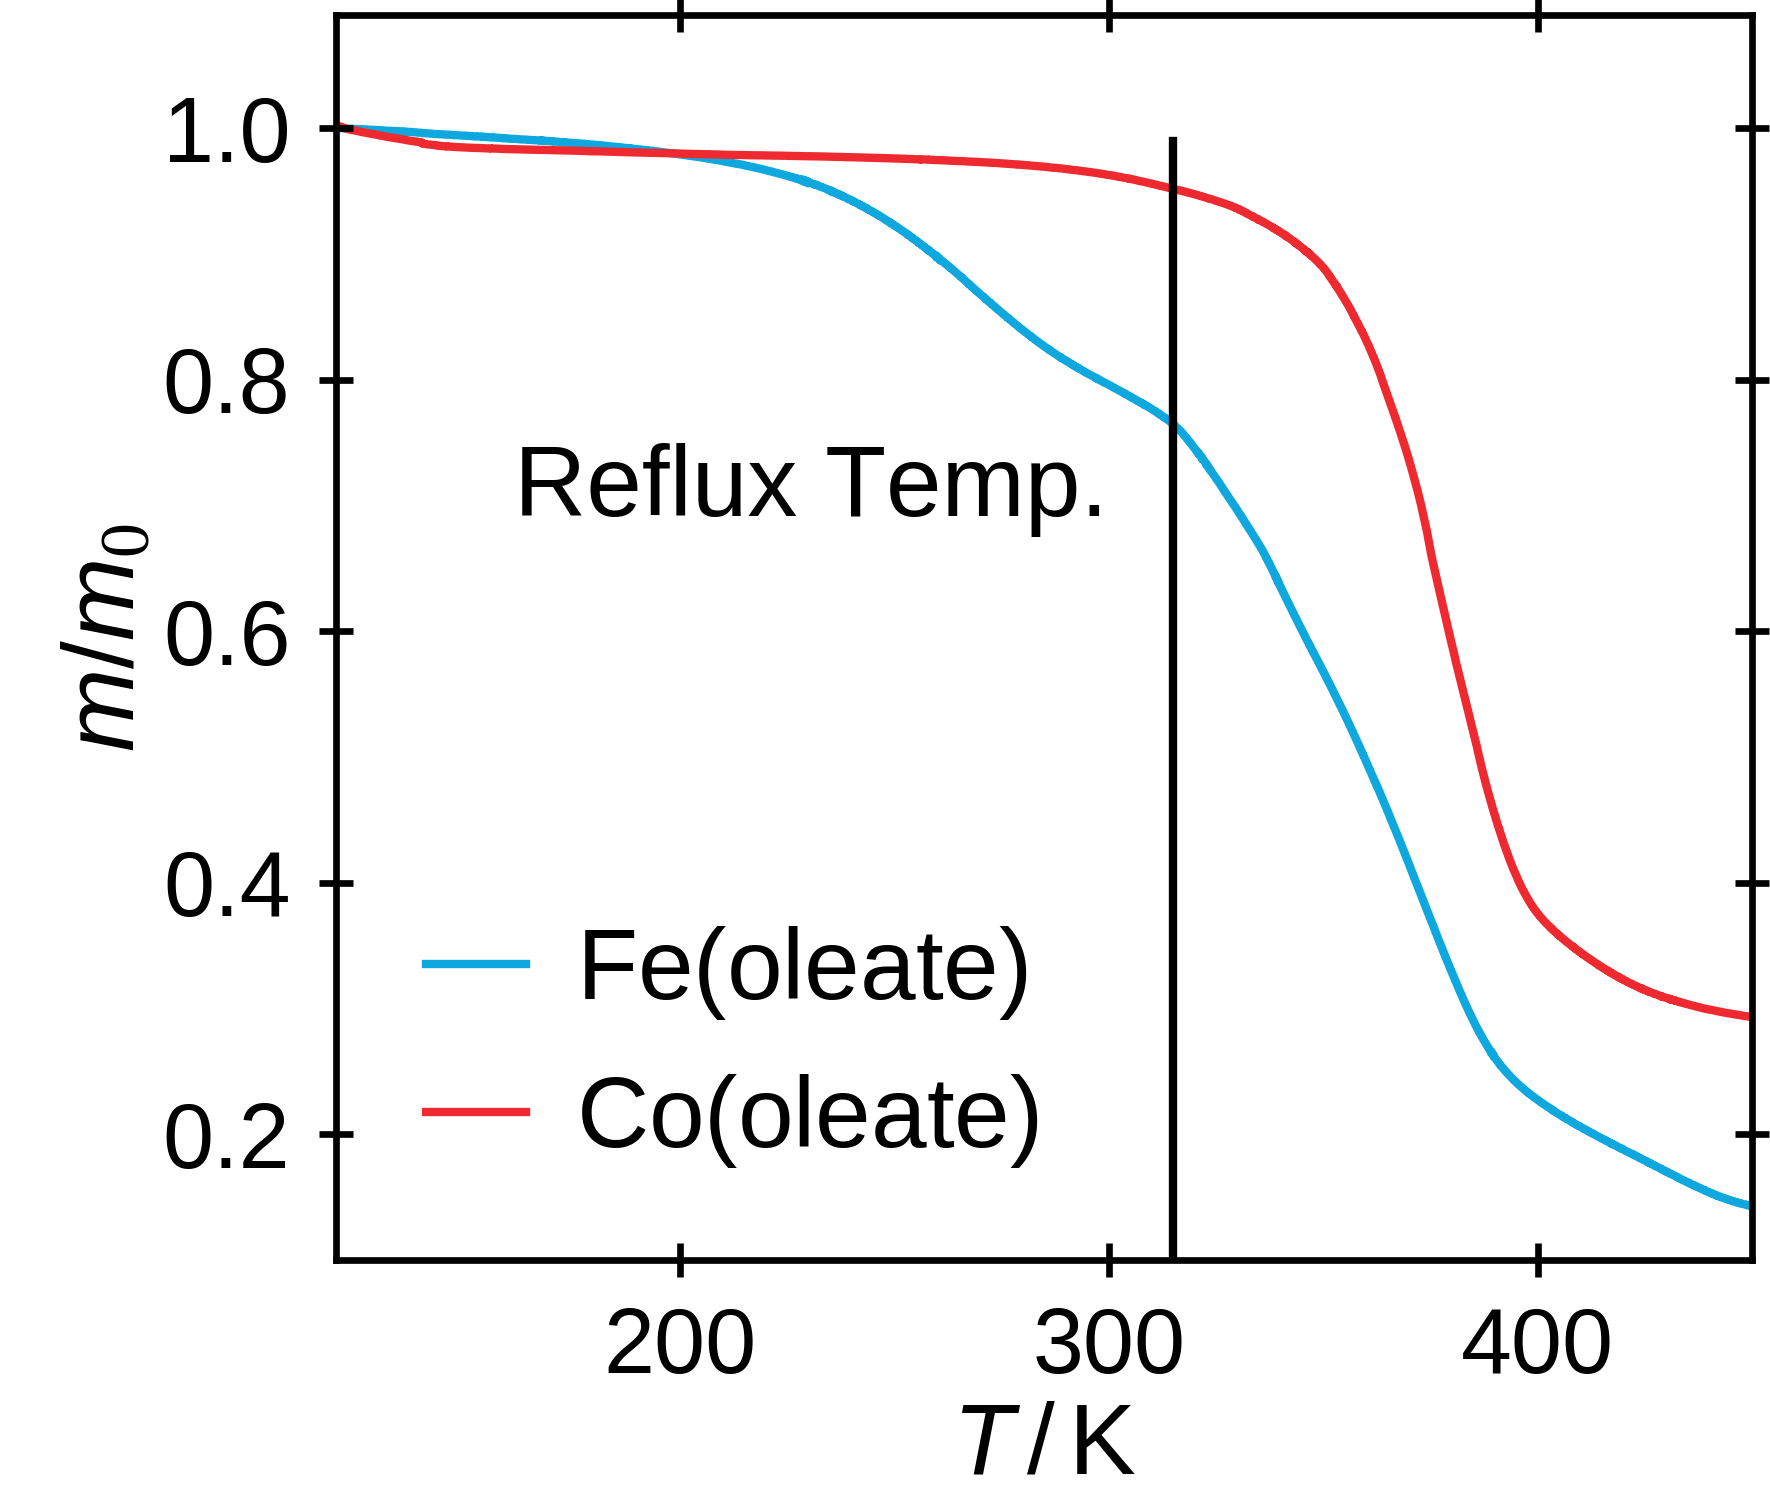
\includegraphics{monolayers_EDX_TGA_OleateTGA}
    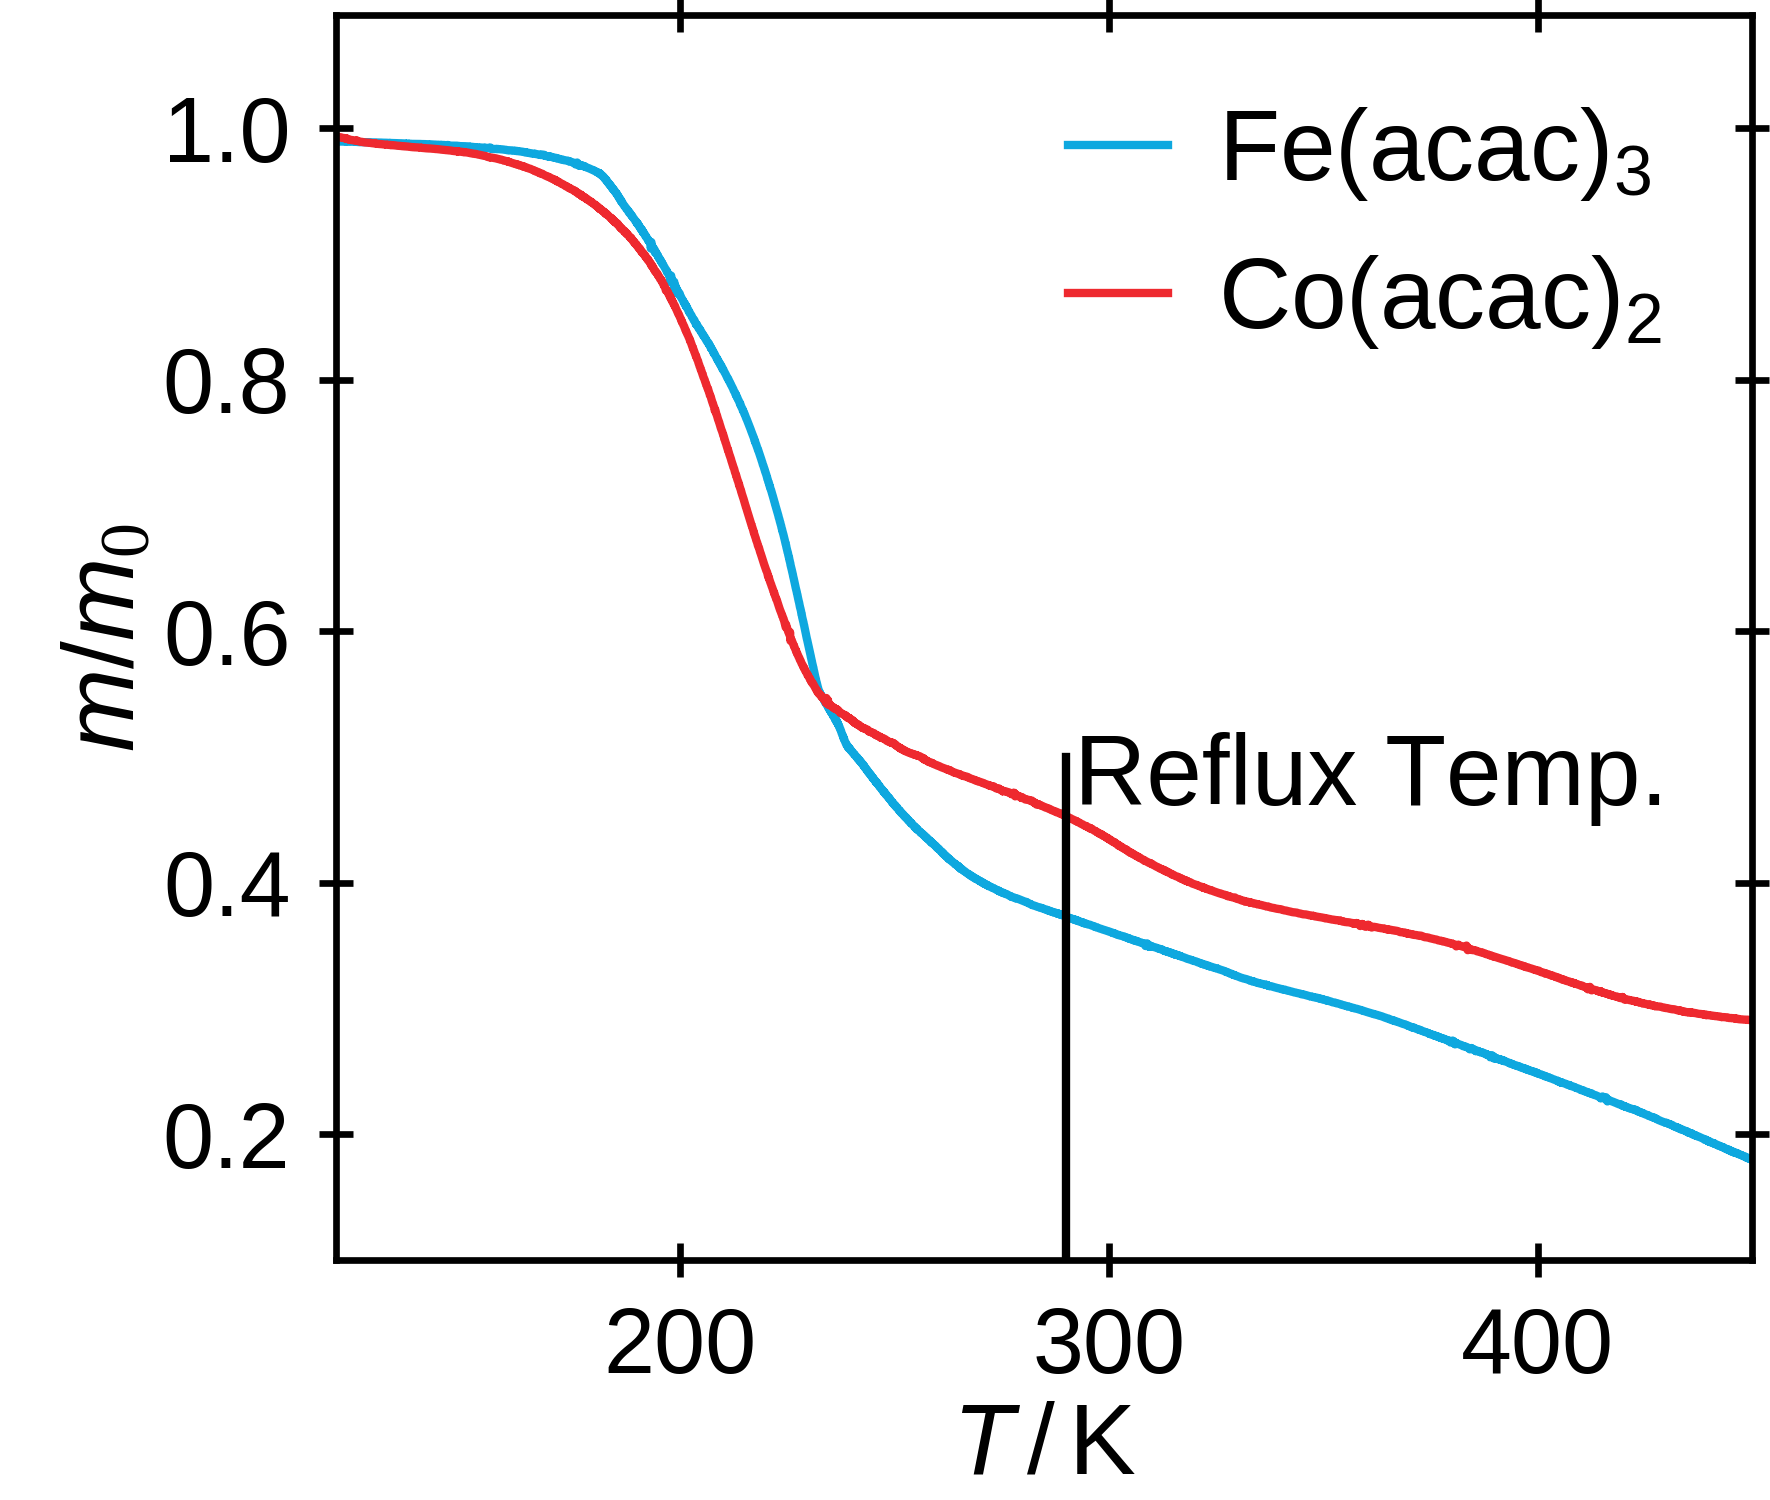
\includegraphics{monolayers_EDX_TGA_AcAcTGA}
    \caption{\label{fig:monolayers:nanoparticle:edx:TGARefluxAcAc}Decomposition  \ch{Fe(acac)_3} and \ch{Co(acac)_2} monitored by thermo-gravimetric analysis.}
    % of \ch{Fe(oleate)} and \ch{Co(oleate)} (left) and
  \end{figure}

  The ratio can be used to deduce the formula unit of the nanoparticles from acetylacetonate.
  The result for both assumptions, a complete occupation of the inverse spinell structure, as typically assumed in literature, and a partially vacant crystal structure with only \ch{Fe^{3+}} are listed in \reftab{tab:monolayers:nanoparticles:edx}.
  For the cases given, the effect of the choice has a small impact on the resulting formula unit.
  For the continuing analysis of the nanoparticles, it is taken that the second formula unit as it is believed that no \ch{Fe^{2+}} is present.

  For Ol-CoFe-C the determination of the formula unit from the EDX result has as additional caveat the dominance of the w\"ustite phase of unknown composition \ch{Fe_x Co_{1-x} O} in the nanoparticle.
  As XRD in \refsec{sec:monolayers:nanoparticle:xrd} however suggests that $97 \%$ of the nanoparticle volme is in a wustite phase, the ratio can be used to approximate the relative composition of iron and cobalt in the w\"ustite phase.

\end{document}